
\section{Management}
\paragraph{}
From the very beginning of the project, we first established the tasks of each person. In order to do so, we each established the areas we wanted to work on.
Each new session was an opportunity for us to share with others our personal progress on the project.

\subsection{Ros and its benefits}
\paragraph{}
For this project, Ros was a great help. Indeed, from the very beginning we've tackled each of these tasks. 
To do this we determined together the graph of the nodes we were going to implement. 
This tool allowed us to avoid any misunderstanding. 
Everyone was able to define what their node subscribed to and what they published. 
This allowed us to reduce the number of common meetings which are very time-consuming.
\subsection{Github}
\paragraph{}
The github platform allowed us to develop files in parallel. 
Indeed, the git software allowed us to access the common kart folder. Git allows us to optimize the development of the project. 
Indeed, on the one hand it allows us to see what others have modified. 
As soon as someone has finished a task that is functional, he pushes on the github and the changes are visible on the online platform. 
Also it allows to always have the most up to date version of the project so that new modifications can be made according to what has been done.

\subsection{agile method}
\paragraph{}
\begin{figure}[ht!]
    \begin{center}
        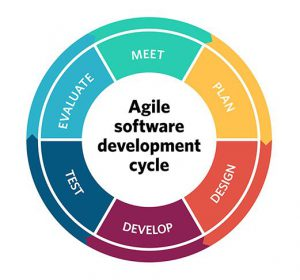
\includegraphics[scale=0.3]{Images/agile_method.jpg}
    \end{center}
    \caption{agile method cycle}
    \label{fig:agile_method}
\end{figure}
The implementation in Ros and github allowed us to set up an agile method. 
Indeed, once the first cycle is completed. 
So the nodes having been created and tested. We started a cycle over. 
So the frequency of meeting was also defined by the frequency of execution of a cycle. This method allowed everyone to have a global vision of the project since the discussion phases were common to everyone.


